\documentclass{beamer}

\usepackage{lipsum}
\usepackage[utf8]{inputenc}
\usepackage[ngerman,english]{babel}
\usepackage{amsmath}
\usepackage{amsthm}
\usepackage{graphicx}
\usepackage{caption}
\usepackage{lmodern}
\usepackage{float}
\usepackage{sidecap}
\usepackage{pgfplots}
\usepackage{pgfplotstable}
\usepackage{tabularcalc}
\usepackage{todonotes}
\usepackage{hyperref}
\usepackage{minted}
\usepackage{siunitx}
\usepackage{subfig}
% \usepackage{tabularx}
% \usepackage{setspace}
\usepackage[customcolors]{hf-tikz}
% \usepackage{url}
% \usepackage{csquotes}
\usepackage{booktabs}
% \usepackage[T1]{fontenc}
% \usepackage[alldates=long]{biblatex}
\graphicspath{ {images/} }
\pgfplotsset{compat=1.12}

\title[Path Tracing]
{Feasibility Study of Real Time Path Tracing}
\subtitle{\textit{Or:} How Much Noise Is Too Much?}
\author[Haase]{Sven-Hendrik Haase \\ \footnotesize Matriculation number: 6341873}
\institute[University of Hamburg]{
    Department of Computer Science\\
    University of Hamburg
}
\subject{Computer Science}

\usetheme{Szeged}
\usecolortheme{seagull}

\begin{document}
\frame{\titlepage}
\begin{frame}
    \frametitle{Table of Contents}
    \footnotesize
    \tableofcontents
\end{frame}

\section{Introduction}

\subsection{Topic}
\begin{frame}
    \frametitle{Topic}
    \begin{block}{Main topic of the thesis}
        When will real time path tracing be viable on consumer grade hardware?
    \end{block}
\end{frame}

\subsection{Motivation}
\begin{frame}
    \frametitle{Motivation}
    \begin{itemize}
        \item Current generation graphics made up of many complex tricks
        \pause
        \item Path tracing is simple in comparison
        \pause
        \item Superior graphics quality
        \pause
        \item Allows for simulation of caustics, global illumination, light dispersion, etc.
        \pause
        \item Real time path tracing appears to be in reach
    \end{itemize}
\end{frame}

\subsection{Leading Question and Goals}
\begin{frame}
    \frametitle{Leading Question and Goals}
    \begin{itemize}
        \item Find out when real time path tracing will be viable
        \item Theoretical indicators (GPU peak FLOPS)
        \item Practical indicators (benchmarks)
        \item Prefer performance to quality
    \end{itemize}
\end{frame}

\section{Real Time Path Tracing Explained}

\subsection{History of Path Tracing}
\begin{frame}
    \frametitle{History of Path Tracing part 1}
    \begin{itemize}
        \item 1968: Ray casting by Arthur Appel
        \item 1980: Ray tracing by Turner Whitted
        \begin{figure}[H]
            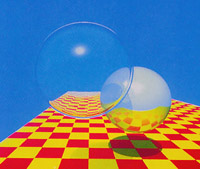
\includegraphics[scale=0.8]{early-raytracing-whitted}
            \centering
            \caption{Turner Whitted's original 1980 image}
        \end{figure}
    \end{itemize}
\end{frame}

\begin{frame}
    \frametitle{History of Path Tracing part 2}
    \begin{itemize}
        \item 1986: Monte Carlo ray tracing (path tracing) by James T. Kajiya
        \item 1996: Bidirectional path tracing by Eric Lafortune
        \item 1997: Metropolis Light Transport by Eric Veach and Leonidas J. Guibas
    \end{itemize}
\end{frame}

\subsection{Physically Based Approach}
\begin{frame}
    \frametitle{Physically Based Approach}
    \begin{block}{Forward path tracing}
        Light source (\(\Rightarrow\) scene interactions) \(\Rightarrow\) observer
    \end{block}
    \begin{block}{Backward path tracing}
        Observer (\(\Rightarrow\) scene interactions) \(\Rightarrow\) light source
    \end{block}
\end{frame}

\subsection{Theoretical Basis}
\begin{frame}
    \frametitle{Theoretical Basis}
    \begin{block}{James Kajiya's rendering equation}
        \scriptsize
        \(
            L_{\text{o}}(\mathbf x,\, \omega_{\text{o}},\, \lambda,\, t) \,=
            \, L_{\text{e}}(\mathbf x,\, \omega_{\text{o}},\, \lambda,\, t) \ +
            \, \int_\Omega f_{\text{r}}(\mathbf x,\, \omega_{\text{i}},\ \omega_{\text{o}},\, \lambda,\, t)
            \, L_{\text{i}}(\mathbf x,\, \omega_{\text{i}},\, \lambda,\, t)\,
            (\omega_{\text{i}}\,\cdot\,\mathbf n)\, \operatorname d \omega_{\text{i}}
        \)
    \end{block}
    \begin{block}{Simplified rendering equation}
        \(
            L_{\text{o}}(\mathbf x,\, \omega_{\text{o}}) \,=
            \, L_{\text{e}}(\mathbf x,\, \omega_{\text{o}}) \ +
            \, \int_\Omega f_{\text{r}}(\mathbf x,\, \omega_{\text{i}},\ \omega_{\text{o}})
            \, L_{\text{i}}(\mathbf x,\, \omega_{\text{i}})\,
            (\omega_{\text{i}}\,\cdot\,\mathbf n)\, \operatorname d \omega_{\text{i}}
        \)
    \end{block}

    \begin{itemize}
        \item Path tracing is a numerical approximate solution to the rendering equation
    \end{itemize}
\end{frame}

\begin{frame}
    \frametitle{Rendering equation breakdown}
\[
    \tikzmarkin[set fill color=red!50!brown!30,set border color=red!40!black]{outgoing}
    L_{\text{o}}(\mathbf x,\, \omega_{\text{o}})
    \tikzmarkend{outgoing}
    \, = \,
    \tikzmarkin[set fill color=cyan!70!lime!30,set border color=cyan!40!black]{emitted}
    L_{\text{e}}(\mathbf x,\, \omega_{\text{o}})
    \tikzmarkend{emitted}
    \ + \,
    \tikzmarkin[set fill color=yellow!50!lime!30,set border color=yellow!40!black]{integral}(0.1,-0.4)(-0.1,0.6)
    \int_\Omega
    \tikzmarkin[set fill color=green!50!lime!30,set border color=green!40!black]{brdf}(0.0,-0.2)(-0.0,0.4)
    f_{\text{r}}(\mathbf x,\, \omega_{\text{i}},\ \omega_{\text{o}})
    \tikzmarkend{brdf}
    \,
    \tikzmarkin[set fill color=blue!50!lime!30,set border color=blue!40!black]{incoming}(0.0,-0.2)(-0.0,0.4)
    L_{\text{i}}(\mathbf x,\, \omega_{\text{i}})
    \tikzmarkend{incoming}
    \,
    \tikzmarkin[set fill color=magenta!100!lime!30,set border color=pink!40!black]{attenuation}(0.0,-0.2)(-0.0,0.4)
    (\omega_{\text{i}}\,\cdot\,\mathbf n)
    \tikzmarkend{attenuation}
    \,
    \operatorname d \omega_{\text{i}}
    \tikzmarkend{integral}
\]
\pause

\(
    \tikzmarkin[set fill color=red!50!brown!30,set border color=red!40!black]{outgoing'}(0.1,-0.15)(-0.1,0.35)
    L_{\text{o}}(\mathbf x,\, \omega_{\text{o}})
    \tikzmarkend{outgoing'}
\)\, is the \textbf{outgoing light} with \(\mathbf x\) being a point on a surface from which the light is
reflected from into direction \(\omega_{\text{o}}\).
\pause

\(
    \tikzmarkin[set fill color=cyan!70!lime!30,set border color=cyan!40!black]{emitted'}(0.1,-0.15)(-0.1,0.35)
    L_{\text{e}}(\mathbf x,\, \omega_{\text{o}})
    \tikzmarkend{emitted'}
\)\, is the \textbf{emitted light} from point \(\mathbf x\).
    \note{Usually surfaces don't emit light themselves unless they are area lights.}
\pause

\smallskip
\(
    \tikzmarkin[set fill color=yellow!50!lime!30,set border color=yellow!40!black]{integral'}(0.1,-0.2)(-0.1,0.35)
    \int_\Omega \, \ldots \, \operatorname d \omega_{\text{i}}
    \tikzmarkend{integral'}
\)\, is the integral over \(\Omega\) which is the hemisphere at \(\mathbf x\) (centered around \(\mathbf n\)). All possible values for \(\omega_{\text{i}}\) are therefore
contained in \(\Omega\).
\pause

\(
    \tikzmarkin[set fill color=green!50!lime!30,set border color=green!40!black]{brdf'}(0.1,-0.15)(-0.1,0.35)
        f_{\text{r}}(\mathbf x,\, \omega_{\text{i}},\ \omega_{\text{o}})
    \tikzmarkend{brdf'}
    \)\, is the \textbf{BRDF} which determines how much light is reflected from
\(\omega_{\text{i}}\) to \(\omega_{\text{o}}\) at \(\mathbf x\).
\pause

\(
    \tikzmarkin[set fill color=blue!50!lime!30,set border color=blue!40!black]{incoming'}(0.1,-0.15)(-0.1,0.35)
        L_{\text{i}}(\mathbf x,\, \omega_{\text{i}})
    \tikzmarkend{incoming'}
\)\, is the \textbf{incoming light} at \(\mathbf x\) from \(\omega_{\text{o}}\).
    \note{It is not necessarily \emph{direct light}. The rendering equation also considers
    \emph{indirect light} which is light that has already been reflected.}
\pause

\smallskip
\(
    \tikzmarkin[set fill color=magenta!100!lime!30,set border color=pink!40!black]{attenuation'}(0.1,-0.15)(-0.1,0.35)
        (\omega_{\text{i}}\,\cdot\,\mathbf n)
    \tikzmarkend{attenuation'}
\)\, is the \textbf{normal attenuation} at \(\mathbf x\).
    \note{The incoming light \(\omega_{\text{i}}\) is
    weakened depending on the cosine of the angle between \(\omega_{\text{i}}\) and the surface normal
    \(\mathbf n\).}
\end{frame}

\subsection{Algorithm}
\begin{frame}[fragile]
    \frametitle{Algorithm part 1}
    \scriptsize
    \begin{minted}[linenos, autogobble]{python}
        max_depth = 5
        scene = [triangle_1, ..., triangle_n]  # Many triangles defined here

        def trace_ray(ray, depth):
            if depth >= max_depth:
                # Return black since we haven't hit anything but we're
                # at our limit for bounces
                return RGB(0, 0, 0) 

            intersection = None
            for triangle in scene:
                intersection = check_intersection(ray, triangle)
                if intersection:  # Break at first intersection
                    break

            if not intersection:
                # If we haven't hit anything, we can't bounce again so
                # we return black
                return RGB(0, 0, 0)
    \end{minted}
\end{frame}

\begin{frame}[fragile]
    \frametitle{Algorithm part 2}
    \scriptsize
    \begin{minted}[linenos, autogobble, firstnumber=20]{python}
            material = intersection.material;
            emittance = material.emittance

            # Shoot a ray into random direction and recurse
            next_ray = Ray()
            next_ray.origin = intersection.position
            next_ray.direction = random_vector_on_hemisphere(intersection.normal)

            # BRDF for diffuse materials
            reflectance_theta = dot(next_ray.direction, intersection.normal)
            brdf = 2 * material.reflectance * reflectance_theta
            reflected = trace_ray(next_ray, depth + 1)

            return emittance + (brdf * reflected)

        for sample in range(samples):
            for pixel in pixels:
                trace_path(ray_from_pixel(pixel), 0)
    \end{minted}
\end{frame}

\subsection{Current State of Technology}
\begin{frame}
    \frametitle{Current State of Technology}
    Projects utilizing real time path tracing:
    \begin{itemize}
        \item Jacco Bikker's and Jeroen van Schijndel's \emph{Brigade Renderer}
        \item David Bucciarelli's \emph{sfera}
        \item Evan Wallace's \emph{WebGL Path Tracer}
    \end{itemize}
\end{frame}

\begin{frame}
    \frametitle{Current State of Technology}
    \begin{figure}[H]
        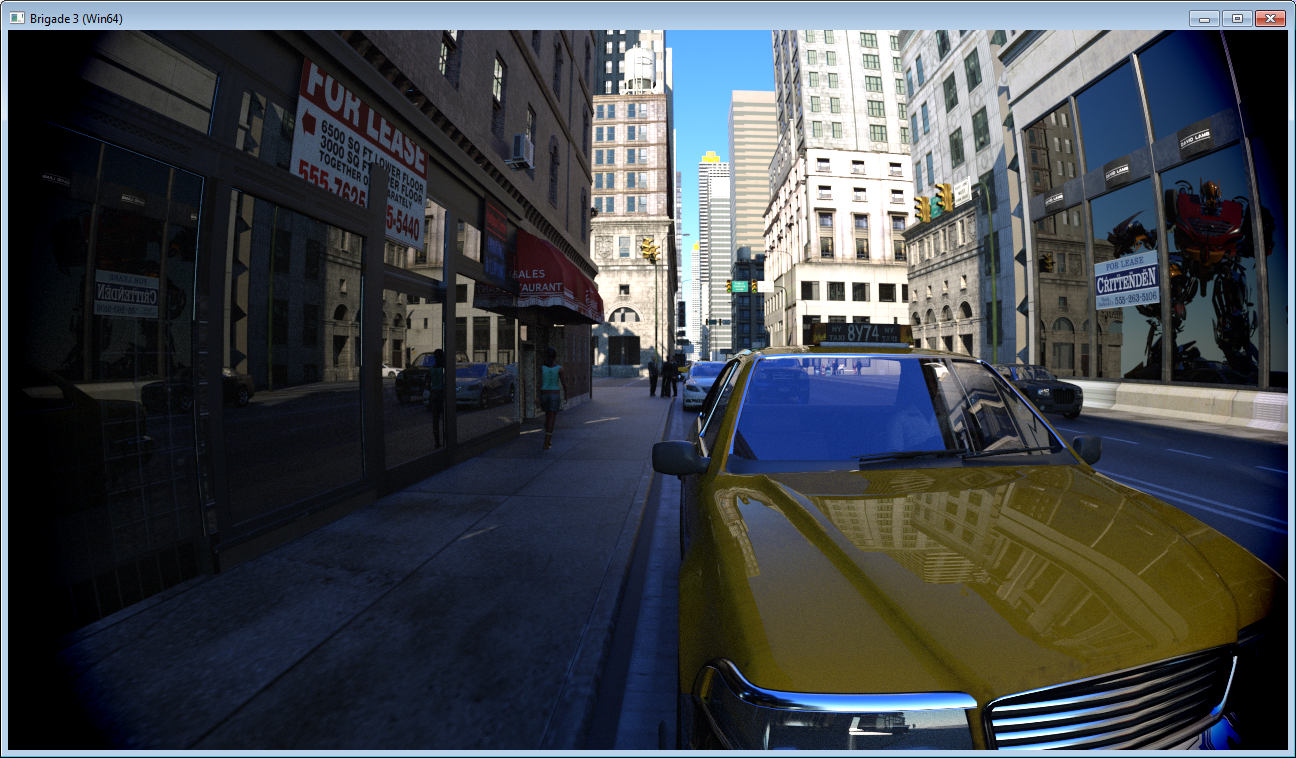
\includegraphics[scale=0.3]{brigade}
        \centering
        \caption{Brigade Renderer}
    \end{figure}
\end{frame}

\begin{frame}
    \frametitle{Current State of Technology}
    \begin{figure}[H]
        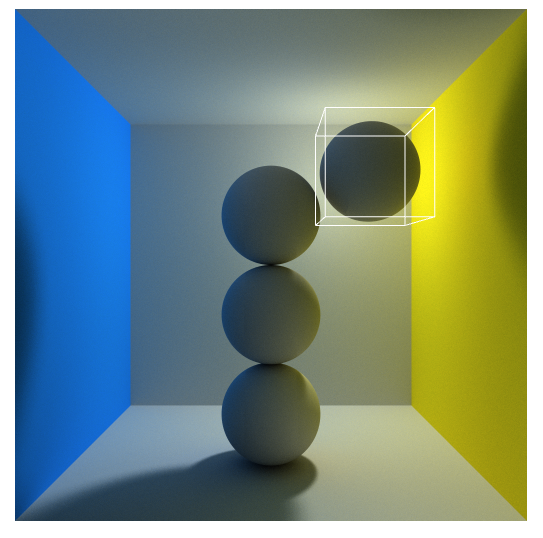
\includegraphics[scale=0.3]{webgl-pathtracer}
        \centering
        \caption{WebGL real time path tracer}
    \end{figure}
\end{frame}

\begin{frame}
    \frametitle{Current State of Technology}
    \begin{figure}[H]
        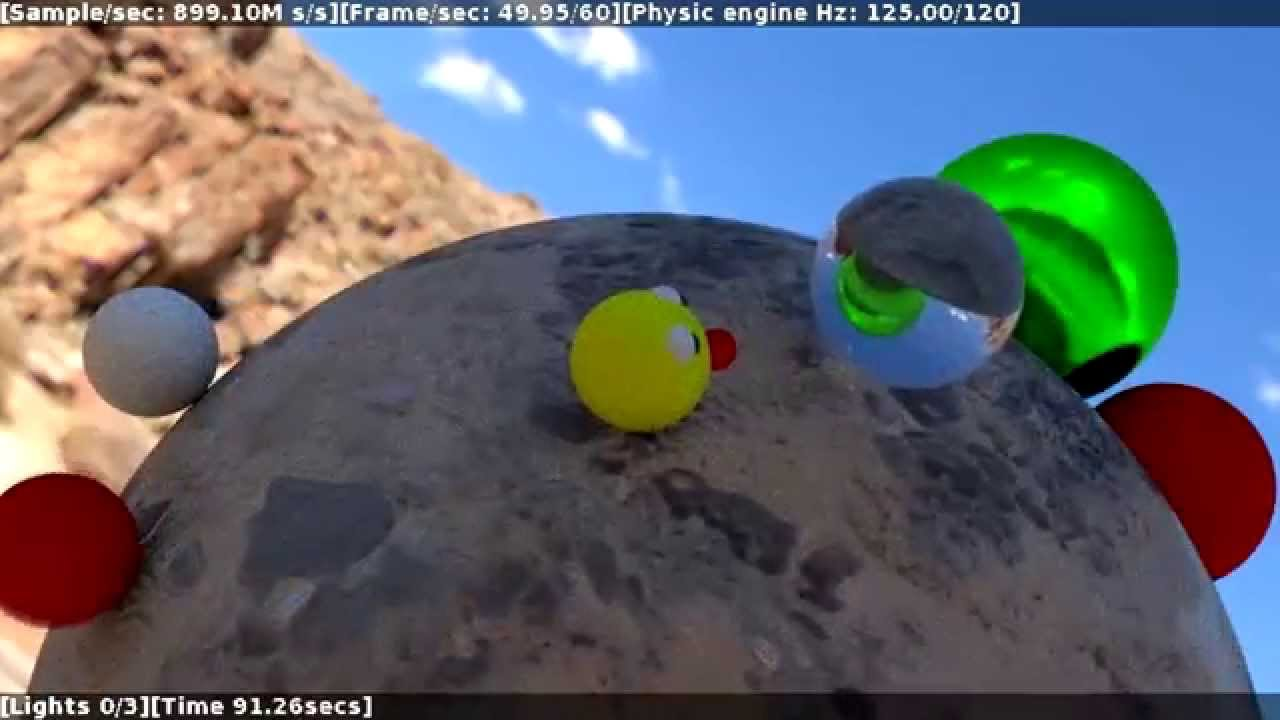
\includegraphics[scale=0.2]{sfera}
        \centering
        \caption{Sfera real time path tracing video game.}
    \end{figure}
\end{frame}

\section{Research}
\subsection{Implementation Design Overview}
\begin{frame}
    \frametitle{Design Overview}
    \pause
    Design goals:
    \begin{enumerate}
        \item \textbf{Speed}\note{In a real time path tracer, rendering speed is of utmost importance as one needs
            to target interactive frame rates at acceptable image quality. The trade-off here is that
            the image is allowed to be grainy as long as it can be shown to the user very quickly.}
        \item \textbf{Ease of implementation}\note{Since the nature and scope of this thesis does not allow for implementing
            the most advanced algorithms, the only constraint for the implementation is for it to be
            good enough for benchmarking.}
        \item \textbf{Interactivity}\note{The path tracer should show off basic interactivity. It should be
            noted, however, that it will probably not reach the requirements for \emph{real time}
            as lined out in chapter \ref{introduction} due to hardware constraints.}
        \item \textbf{Portability}\note{The software should run on different GPUs as well CPUs with different
            memory and core configurations respectively with minimal effort. It should therefore be
            written with this portability in mind to make it easier to adapt.}
        \item \textbf{Maintainability}\note{The software should be easy to understand, well-documented and
            easy to debug. Code should be commented where necessary.}
    \end{enumerate}
\end{frame}

\begin{frame}
    \frametitle{Design Overview}
    Components:
    \begin{itemize}
        \item Random number generation
            \note{Solid and fast function for pseudo random number generation.}
        \item Camera
            \note{A structure that keeps all camera data as well as some functions to do coordinate
            transformations.}
        \item Material system
            \note{The path tracer has to support at least four materials: Emissive,
            diffuse, glossy and glass. Each of them should at least provide their BRDF.}
        \item AABBs
            \note{A simple way to represent AABBs.}
        \item Triangles
            \note{The only kind of primitive that materials can be applied unto and in fact the
            only kind of geometry that is rendered.}
        \item Shapes and geometry
            \note{A way to generate basic geometric shapes should be provided. No
            mechanism for loading externally defined models is necessary.}
        \item Scene
            \note{A way to efficiently save an arbitrary number of shapes. At first this should be
            implemented as a flat list. Optionally, a more efficient data structure can be
            implemented.}
        \item Intersection/Scene lookup
            \note{Implemented as a ray intersection function for each supported primitive
            (which in this case means ray-AABB intersection and ray-triangle intersection).}
        \item Viewer
            \note{An interactive viewport that shows off progressive rendering with a sample
            scene.}
    \end{itemize}
\end{frame}

\begin{frame}
    \frametitle{Design Overview}
    Materials:
    \begin{itemize}
        \item Emissive
        \item Diffuse
        \item Glass
        \item Glossy
    \end{itemize}
\end{frame}

\subsection{Results}
\begin{frame}[shrink]
    \frametitle{Visual Results}
    \pause
    \begin{figure}[H]
        \subfloat[\(n = 1\)]{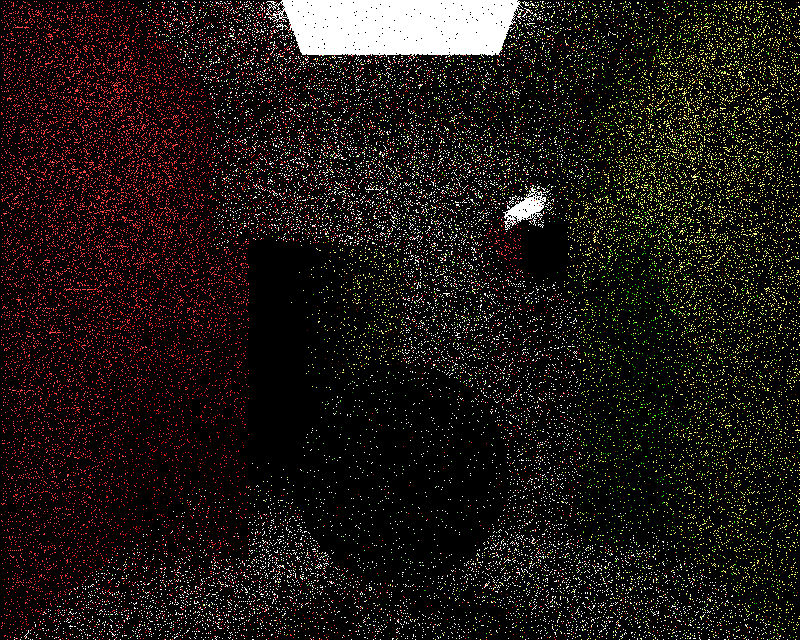
\includegraphics[scale=0.10]{trac0r-1.png}}
        \subfloat[\(n = 2\)]{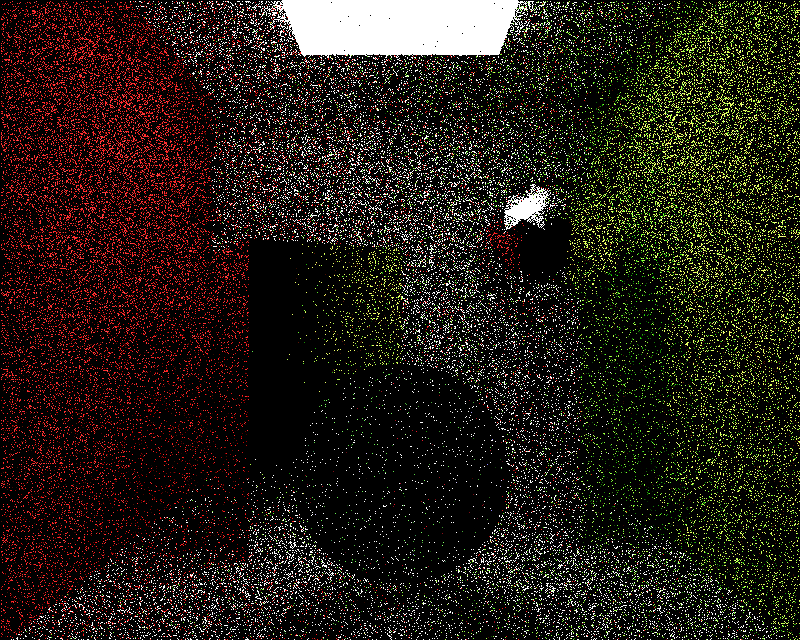
\includegraphics[scale=0.10]{trac0r-2.png}}
        \subfloat[\(n = 3\)]{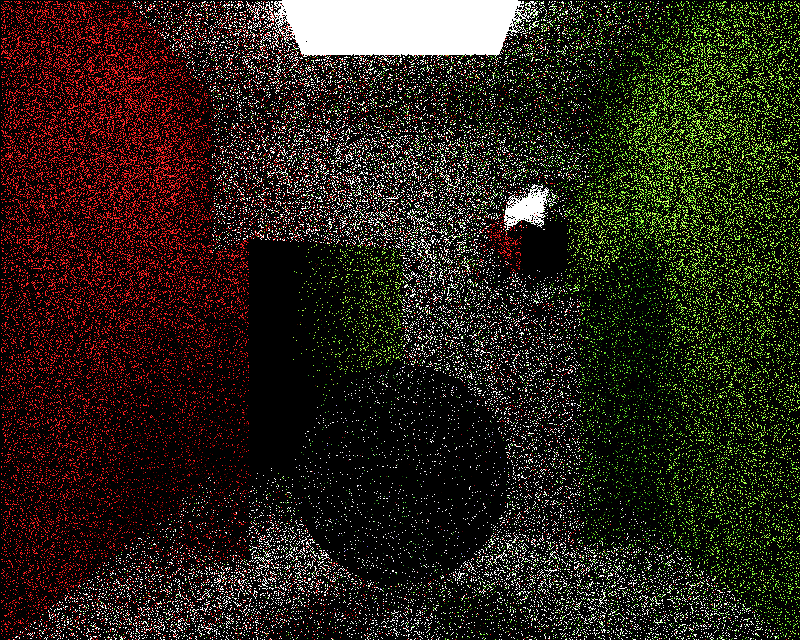
\includegraphics[scale=0.10]{trac0r-3.png}}
        \subfloat[\(n = 4\)]{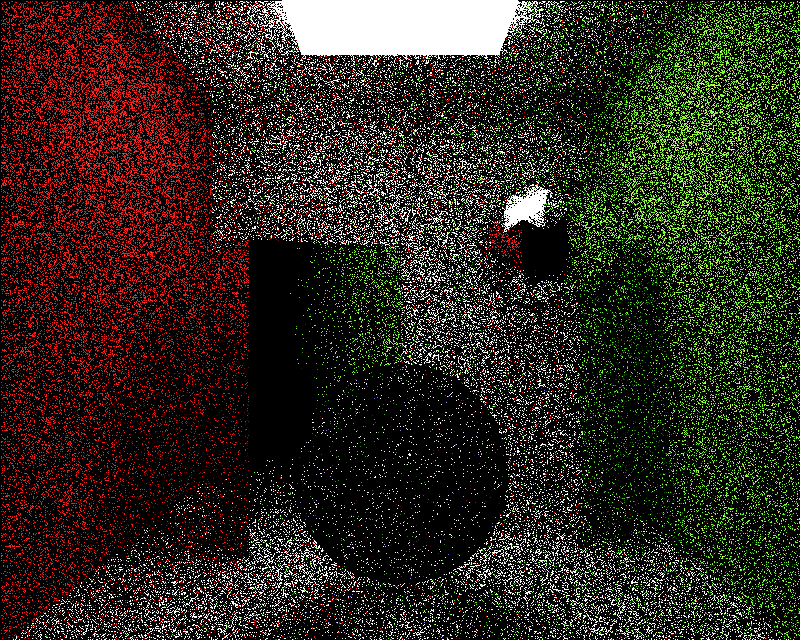
\includegraphics[scale=0.10]{trac0r-4.png}}
        \centering

        \subfloat[\(n = 10\)]{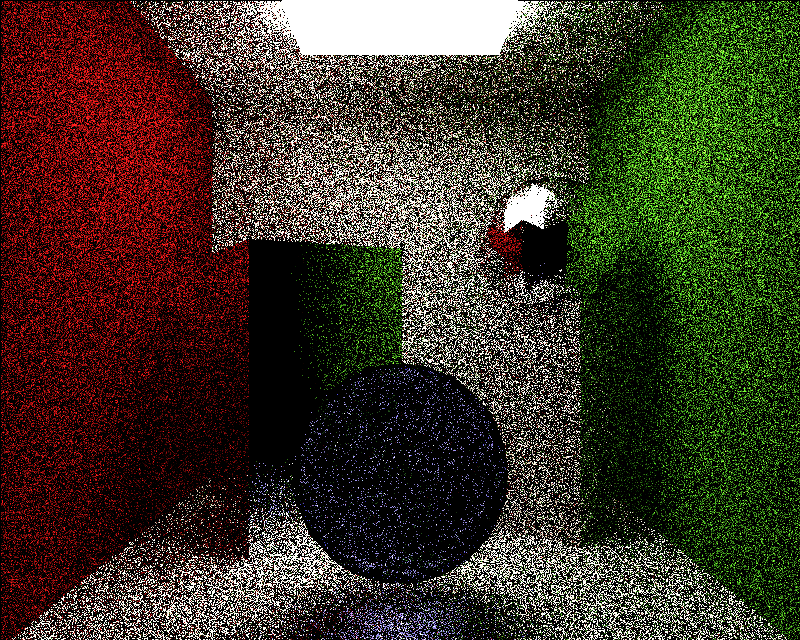
\includegraphics[scale=0.10]{trac0r-10.png}}
        \subfloat[\(n = 20\)]{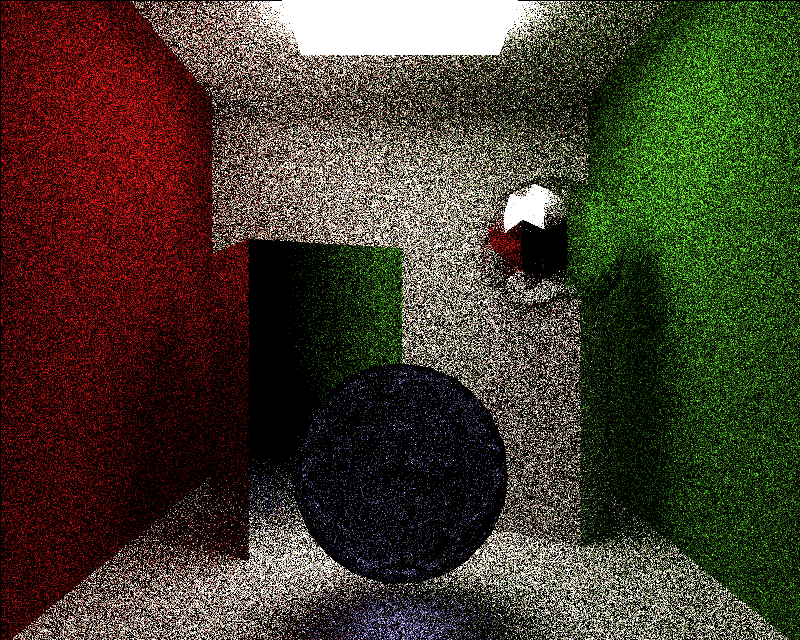
\includegraphics[scale=0.10]{trac0r-20.png}}
        \subfloat[\(n = 50\)]{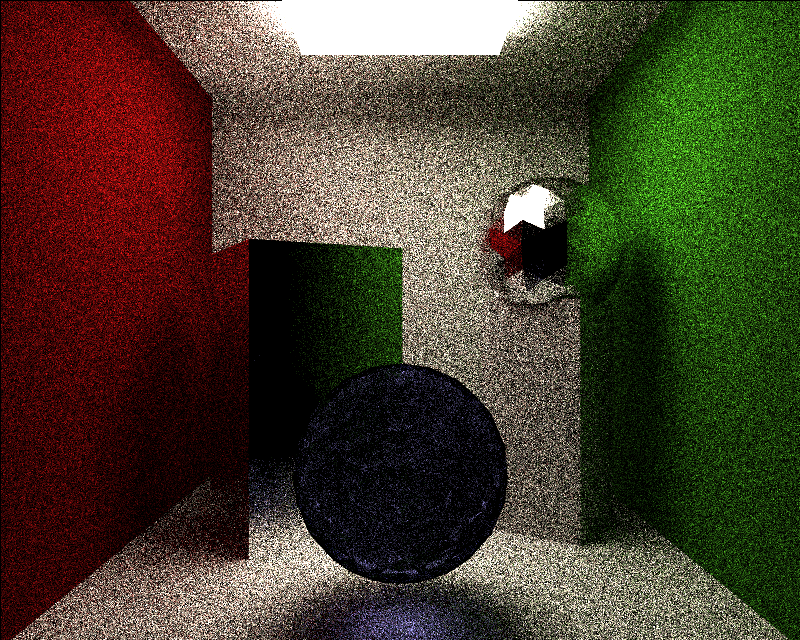
\includegraphics[scale=0.10]{trac0r-50.png}}
        \subfloat[\(n = 100\)]{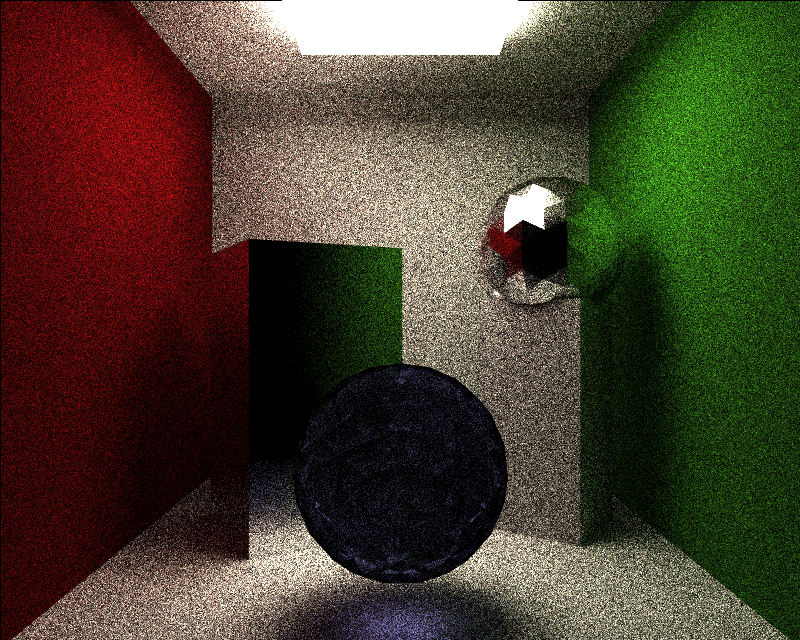
\includegraphics[scale=0.10]{trac0r-100.png}}
        \centering
    \end{figure}
\end{frame}

\begin{frame}[shrink]
    \frametitle{Visual Results}
    \begin{figure}[H]
        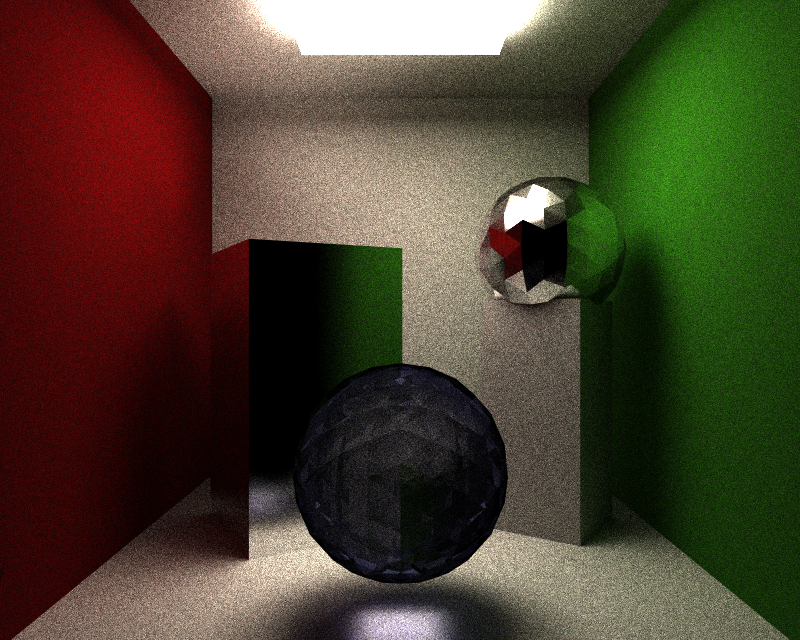
\includegraphics[scale=0.5]{trac0r-5000.png}
        \centering
        \caption{trac0r\_viewer after integrating for 5000 frames.}
    \end{figure}
\end{frame}

\begin{frame}[shrink]
    \frametitle{Visual Results}
    \begin{figure}[H]
        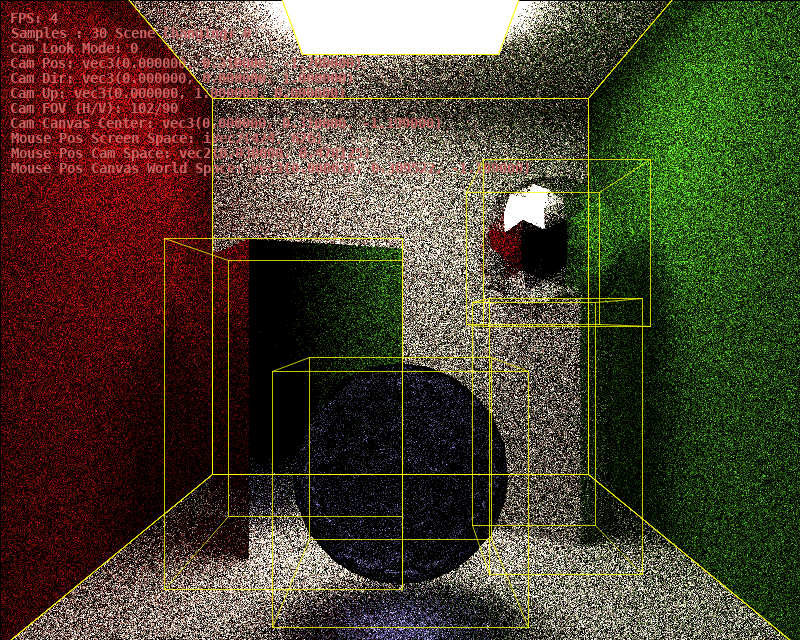
\includegraphics[scale=0.5]{trac0r-debug1.png}
        \centering
        \caption{trac0r\_viewer debug view.}
    \end{figure}
\end{frame}

\begin{frame}[shrink]
    \frametitle{Visual Results}
    \begin{figure}[H]
        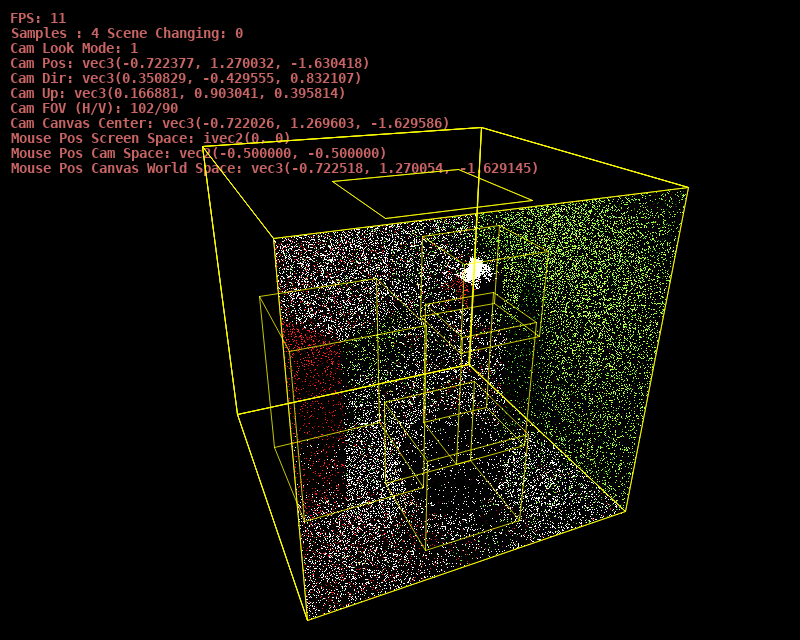
\includegraphics[scale=0.5]{trac0r-debug2.png}
        \centering
        \caption{trac0r\_viewer debug view while interactively navigating the scene.}
    \end{figure}
\end{frame}

\begin{frame}
    \frametitle{Visual Results}
    Live presentation!
\end{frame}

\subsection{Evaluation}
\begin{frame}[shrink]
    \frametitle{Evaluation}
    \pause
    \begin{figure}[H]
        \begin{tikzpicture}
            \begin{axis}[
                    title={Performance in correlation to scene complexity},
                    xlabel={Triangles},
                    ylabel={FPS},
                    legend pos=north east,
                    ymajorgrids=true,
                    grid style=loosely dashed,
                    smooth,
                    cycle list name=exotic,
                    x tick label style={align=center, rotate=45},
                    width=\textwidth
                ]

                \addplot
                    coordinates {
                        (56,16.9)
                        (116,13.9)
                        (356,7.4)
                        (1316,2.6)
                        (5156,0.72)
                    };

                \addplot
                    coordinates {
                        (56,26)
                        (116,19.5)
                        (356,8.9)
                        (1316,2.8)
                        (5156,0.73)
                    };

                \addplot
                    coordinates {
                        (56,17.6)
                        (116,15.6)
                        (356,9.5)
                        (1316,3.7)
                        (5156,1.0)
                    };

                \addplot
                    coordinates {
                        (56,24)
                        (116,21.8)
                        (356,14)
                        (1316,5.8)
                        (5156,1.7)
                    };

                \addplot
                    coordinates {
                        (56,24)
                        (116,22.4)
                        (356,15)
                        (1316,6.2)
                        (5156,1.83)
                    };
                \legend{NVIDIA Geforce GTX 660, NVIDIA Geforce GTX 570,
                    NVIDIA Geforce GTX 960, NVIDIA Geforce GTX 970,
                NVIDIA Geforce GTX 980}
            \end{axis}
        \end{tikzpicture}
        \centering
        \note{Scene complexity benchmark on a variety of graphics cards. It was benchmarked at
        a resolution of 800x600.}
    \end{figure}
\end{frame}

\begin{frame}
    \frametitle{Evaluation}
    \begin{table}[H]
        \centering
        \begin{tabular}{l | r | r | r}
            GPU                     & Average FPS   & GFLOPS & \(\frac {\text{Average FPS}}{GFLOPS}\)\\
            \midrule
            NVIDIA Geforce GTX 660  & 8.3           & 1881.6 & \num{4.4e-3} \\
            NVIDIA Geforce GTX 570  & 11.6          & 1405.4 & \num{8.6e-3} \\
            NVIDIA Geforce GTX 960  & 9.5           & 2308   & \num{4.1e-3} \\
            NVIDIA Geforce GTX 970  & 13.5          & 3494   & \num{3.9e-3} \\
            NVIDIA Geforce GTX 980  & 13.9          & 4612   & \num{3.0e-3}
        \end{tabular}
        \caption{Tested GPU performance and GFLOPS.}
    \end{table}
\end{frame}

\begin{frame}[shrink]
    \frametitle{Evaluation}
    \begin{figure}[H]
        \begin{tikzpicture}
            \begin{axis}[
                    title={GFLOPS of highend consumer desktop GPUs by year},
                    xlabel={Year of release},
                    ylabel={Peak single precision performance [GFLOPS]},
                    xmin=2005,
                    xmax=2020,
                    ymin=0,
                    ymode=log,
                    log ticks with fixed point,
                    legend pos=north west,
                    ymajorgrids=true,
                    xmajorgrids=true,
                    legend cell align=left,
                    grid style=loosely dashed,
                    extra y ticks={500, 2500, 5000, 20000, 40000},
                    x label style={below=5mm},
                    extra y tick style={log identify minor tick positions=false},
                    x tick label style={align=center, rotate=45, /pgf/number format/1000 sep={}},
                    width=12cm
                ]

                \addplot+[
                        green!60!black,
                        only marks,
                        mark options={green!60!black},
                        point meta=explicit symbolic,
                        nodes near coords
                    ]
                    coordinates {
                        (2006,518) [\tiny Geforce 8800 GTX]
                        (2008,648) [\tiny Geforce 9800 GTX]
                        (2008,933) [\tiny Geforce GTX 280]
                        (2010,1345) [\tiny Geforce GTX 480]
                        (2010,1581) [\tiny Geforce GTX 580]
                        (2012,3090) [\tiny Geforce GTX 680]
                        (2013,3977) [\tiny Geforce GTX 780]
                        (2014,4612) [\tiny Geforce GTX 980]
                    };

                \addplot+[
                        red,
                        only marks,
                        mark options={red},
                        point meta=explicit symbolic,
                        nodes near coords
                    ]
                    coordinates {
                        (2007,384) [\tiny Radeon HD 2900 PRO]
                        (2008,1200) [\tiny Radeon HD 4870]
                        (2009,2720) [\tiny Radeon HD 5870]
                        (2011,2703) [\tiny Radeon HD 6970]
                        (2012,3789) [\tiny Radeon HD 7970]
                        (2013,4849) [\tiny Radeon R9 290]
                        (2015,7168) [\tiny Radeon R9 Fury]
                    };

                \addplot+[
                        gray,
                        smooth,
                        mark=none,
                        densely dashed,
                        thick
                    ]
                    coordinates {
                        (2004,250*0.7)
                        (2006,500*0.7)
                        (2008,1000*0.7)
                        (2010,2000*0.7)
                        (2012,4000*0.7)
                        (2014,8000*0.7)
                        (2016,16000*0.7)
                        (2018,32000*0.7)
                        (2020,64000*0.7)
                    };
                    % Formula is: 250*2^(0.5(x-2004))*0.7 x is from 2004 to 2020
                    \legend{NVIDIA GPUs, AMD GPUs, Mean GFLOPS}
                \end{axis}
            \end{tikzpicture}
            \centering
        \end{figure}
    \end{frame}

    \section{Conclusion and Outlook}
    \subsection{Conclusion}
    \begin{frame}
        \frametitle{Conclusion}
        \begin{itemize}
            \item Recall the goal: When will real time path tracing be viable on commodity hardware?
            \pause
            \item Data and research suggests viability in \(\approx 4\) years
        \end{itemize}
    \end{frame}

    \subsection{Outlook}
    \begin{frame}
        \frametitle{Outlook}
        Many venues for improvement:
        \pause
        \begin{itemize}
            \item Overall: Faster hardware
                \pause
            \item Software: Memory access optimizations
                \pause
            \item Intersection: Acceleration Data Structure (BVH, kd-tree)
                \pause
            \item Convergence: Bidirectional path tracing + Multiple Importance Sampling
                \pause
            \item Image filtering: Bilateral filter
                \pause
            \item Research: Who knows?
        \end{itemize}
        \pause
        \(\Longrightarrow\) Real time path tracing possible within 4 years
    \end{frame}

    \begin{frame}
        \frametitle{Fin}
        Thank you for your attention.
    \end{frame}
    \end{document}
